\begin{minted}[breaklines]{latex}
C\# ist eine objektorientierte Programmiersprache, die im Auftrag von Microsoft entwickelt wurde und die es bereits seit 2001 gibt. In \cref{fig:csharp} seht ihr das Logo der Programmiersprache. 
	
\begin{figure}[H]
	\caption{Das Logo der Programmiersprache C\#}
	\label{fig:csharp}
	\centering
	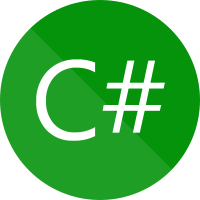
\includegraphics[width=2cm]{exercises/references/csharp.png}
\end{figure}

\cref{lst:csharphelloworld} zeigt ein Programm, das den Text \enquote{Hello LaTeX friends!} auf der Konsole ausgibt. Ähnlich wie bei Java werden auch in C\# Klassen und eine Main-Methode verwendet, um eine ausführbare Anwendung zu bauen. 
	
\begin{listing}[H]
	\caption{Ein einfaches Programm in der Programmiersprache C\#}
	\label{lst:csharphelloworld}
	\inputminted[breaklines, linenos=true]{csharp}{exercises/references/HelloLateXFriends.cs}
\end{listing}
\end{minted}



	


